\documentclass{article} % For LaTeX2e
\usepackage{nips12submit_e,times}
%\documentstyle[nips12submit_09,times,art10]{article} % For LaTeX 2.09
\usepackage{amsmath,amsthm,amssymb, dsfont}
\usepackage{pgf}
\usepackage{tikz}
\usetikzlibrary{arrows,automata}

\title{Infectious Knowledge in a Collaborative News Site}


\author{
Eliana Feasley\\
Department of Computer Science\\
University of Texas at Austin\\
\texttt{elie@cs.utexas.edu} \\
\And
Wesley Tansey\\
Department of Computer Science\\
University of Texas at Austin\\
\texttt{tansey@cs.utexas.edu} \\
}

\newcommand{\fix}{\marginpar{FIX}}
\newcommand{\new}{\marginpar{NEW}}
\def\c{\textbf{ Cite }}
\nipsfinalcopy

\begin{document}

\maketitle

\begin{abstract}
In recent years, the attention paid to cascading information in soical networks has been increasing in a fashion itself comparable to a social cascade. This makes sense - the way that information infects different spaces of ideas has applications to basic graph theory\c, epidemiology\c, future prediction\c, and marketing\c. In this paper, we examine the dynamics of information spread across subcommunities with overlapping networks in both the social news collaborative filering site reddit\footnote{\texttt{www.reddit.com}} and in several data mining conferences. Both of these are structured such that it is possible to track how ideas spread over time, and to discover semi-explicit communities and the connections between them.
\end{abstract}

\section{Introduction}
\label{intro}
Information online travels across networks in a variety of configurations, and it is easy to see information spreading across them. Past work such as \c \c and \c all illustrate examples of phrases or terms spreading rapidly across networks.
This is an extension of the work in \cite{netinf}, in which the authors learn the structure of a graph from observing cascades. We assume the graph is fully connected, and predict the state of a cascade given the inferred weights on the graph. 

In this paper, we explore how modeling this machanism as a timeseries can help us both to predict future topics and to discover the strengths of the connections between communities. Section \ref{data} explains the structure of the data and the domains from which they are drawn. Section \ref{cascades} delves into past work on cascades in networks. Sections \ref{experiments} and \ref{results} explain the experiments and results respectively, and Section \ref{discussion} explores the broader implications of our results and some future work. 

\section{Social Cascades}
\label{cascades}

In \cite{info_contag} the authors use the explicit struture of networks - observing following and friendship relationships in order to explore the effect of actual, instead of inferred, network structure on information cascades. They observe that the popularity of stories peaks with an age of about one day, and then subsides. 

A unique aspect of open networks like reddit, digg, publications, \&c is that it is possible for information to latently travel quicly, as opposed toin closed, action oriented networks like the one described in \cite{viral_dynamics}, where information, which must individually be spread from one email to another, peters out quickly.

In \cite{twitter_trend}, the authors identify \textit{bursty} keywords that suddently appear, and attempt to align them with trends - entire topics that are becoming more popular. They do this by analyzing new bursts in the queue. One thing we can do in this paper is look at each sub as a queue and see if bursts in one are followed by bursts in another.


\subsection{Problem Statement}

Given nodes $\mathcal{D}$ with overlapping connections $\mathcal{C}$ via shared users, predict topic vector $v_{d,t+1}$ in document collection $d$ at time $t+1$ given the topics $V$ in all documents at time $t$?


Following the model in \cite{influential}, we refer to a node as \textit{contagious} for a given phrase if it has had that phrase trend internally within the last timestep. A node that contains a previously trending phrase can be viewed as having become \textit{infected.} 

% figure showing the number of uses of some phrase over several time-steps

\subsection{Problem Structure}

$$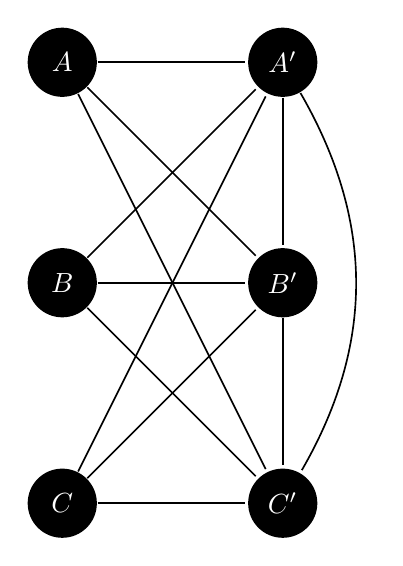
\begin{tikzpicture}[-,>=stealth',shorten >=1pt,auto,node distance=2.8cm,
                    semithick]
  \tikzstyle{every state}=[fill=black,draw=none,text=white]

  \node[state] (A)                    {$A$};
  \node[state]         (B) [below of=A] {$B$};
  \node[state]         (C) [below of=B] {$C$};
  \node[state]         (A1) [right  of=A] {$A'$};
  \node[state]         (B1) [right of=B] {$B'$};
  \node[state]         (C1) [right of=C] {$C'$};


  \path (A) edge        node {} (A1)
        (A) edge        node {} (B1)
        (A) edge        node {} (C1)
        (B) edge        node {} (A1)
        (B) edge        node {} (B1)
        (B) edge        node {} (C1)
        (C) edge        node {} (A1)
        (C) edge        node {} (B1)
        (C) edge        node {} (C1)
        (A1) edge        node {} (B1)
        (A1) edge [bend left] node {} (C1)
        (B1) edge        node {} (C1);
\end{tikzpicture}
$$

\subsection{Detecting Infections}
\label{infections}

To detect infections, we use Pointwise Mutual Information \cite{pmi} to identify salient bigrams in each site in each timestep. Whenever these occur multiple times across the entire dataset, they may be infections. We examine the occurences of each ngram to see if it appears in bursts, and if it does, we designate it an infection.


\subsection{Learning Parameters}

We used the method for finding the MLE estimate in triangulated graphs described in \cite{wainwright} to learn the weights of our edges.


\section{Datasets}
\label{data}

Our algorithm is evaluated on three datasets: a reddit dataset scraped from reddit.com, a stack-exchange dataset, and a synthetic dataset.

\subsection{Reddit}
Reddit is divided into thousands of \textit{subreddits}, each of which is targeted towards specialty interests. There is a many-to-many relationship between users and subreddits, with most users active in many subreddits and most subreddits populated with many users.

We looked at the top 20 subreddits in terms of popularity, and as these are so active, we set our timestep to be six hours. For each timestep, we formed a document of all of the post titles present during that time. A contagion was defined as described in \ref{infections}.


\subsection{StackExchange}

\subsection{Synthetic Dataset}


% Figure showing some structure of connections between reddits

% Figure showing some structure of connections between conferences

\section{Experiments}
\label{experiments}

We conducted three sets of experiements, on the \texttt{reddit} dataset, the \texttt{StackExchange} dataset, and the synthetic dataset. Each of these was similar, in that we used $n$-fold cross-validation to predict cascades with our algorithm, and with the edge weights learned by NetInf.




\section{Results}
\label{results}

% predicted prevalence of phrase based on network vs based on entire thing

% predicted network structure given phrases


\section{Discussion}
\label{discussion}


\bibliography{sources}{}
\label{refs}
\bibliographystyle{plain}

\end{document}